\documentclass[11pt,a4paper]{article}
\usepackage[margin=24mm,top=20mm,bottom=19mm]{geometry}
\usepackage[T1]{fontenc}
\usepackage{lmodern,tikz,hyperref}
\definecolor{ink}{HTML}{203B39}\definecolor{sea}{HTML}{237466}\definecolor{gold}{HTML}{E9B858}\definecolor{pale}{HTML}{E5F1EC}
\hypersetup{colorlinks=true,urlcolor=sea,pdftitle={How complex is your neural network?}}
\setlength{\parindent}{0pt}\setlength{\parskip}{6pt}\raggedright
\newcommand{\head}[1]{\par\medskip{\large\sffamily\bfseries\color{sea}#1}\par}
\begin{document}
{\fontsize{26}{30}\selectfont\sffamily\bfseries\color{ink} How complex is your neural network?\par}
{\large\itshape Counting parameters is the wrong answer}\par
Classical statistics gives us familiar tools for choosing a model. AIC and BIC weigh how well it fits against a penalty for its flexibility. Hand them a large neural network and a simple question gets harder. What should count as flexibility when a network has more weights than training examples?
\head{The parameter-count trap}
Ask how big a neural network is and you will hear a number of parameters. Ask why it works on data it has never seen, and that number stops helping. Two networks can have exactly the same number of weights. One can still be much easier to describe.

Think of two books. One has a thousand pages, but every page repeats the same sentence. The other is a single page of random characters. You could dictate the thick book over the phone in a few seconds. Try doing that with the thin one.
\begin{center}
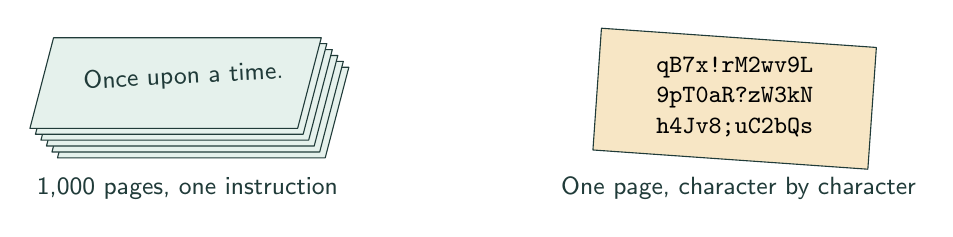
\begin{tikzpicture}[x=1cm,y=1cm,font=\sffamily\small,line join=round]
\foreach \n in {0,...,5}{\begin{scope}[shift={(-.07*\n,.075*\n)}]
\filldraw[fill=pale,draw=ink] (0,0)--(3.4,0)--(3.7,1.15)--(.3,1.15)--cycle;\end{scope}}
\node[ink,rotate=3] at (1.6,1.02){Once upon a time.};
\node[below,ink] at (1.65,-.12){1,000 pages, one instruction};
\begin{scope}[shift={(6.8,.1)},rotate=-4]
\filldraw[draw=ink,fill=gold!35] (0,0) rectangle (3.5,1.55);
\node[align=left,font=\ttfamily\small] at (1.75,.8){qB7x!rM2wv9L\\9pT0aR?zW3kN\\h4Jv8;uC2bQs};\end{scope}
\node[below,ink] at (8.65,-.12){One page, character by character};
\end{tikzpicture}
\end{center}
\head{Complexity as description length}
Suppose you have the inputs and I have the labels. I can send you my model, then use its predictions to tell you which label each input got. A label the model gives probability one half costs one bit in an ideal code. A label it gives probability one eighth costs three. A confident mistake makes the message longer.

How many bits did we spend altogether? The minimum description length (MDL) principle favours the shortest complete explanation. In a two-part code we pay once for the model and again for the labels given the model you receive.
\head{Many roads, different meanings}
An information criterion such as BIC asks how much the fit improves for the number of parameters we use. A prequential code asks how many bits we would spend predicting the next labels as we learn. A compression bound asks how large the error on new examples could be if a smaller network preserves the original network's predictions closely enough. Before comparing two numbers, it helps to know which question each one answers.
\newpage
\head{What we are building}
Our project, DL Complexity, is a PyTorch library that lets you ask each of these questions through the same interface. Each answer tells you its units, what went into the calculation and which assumptions it relies on. You can reuse a checkpoint and choose the measure that fits your question.

Take the two-part code. We used a fixed network to generate 20,000 labels across four classes. We gave its weights between one and sixteen bits per index, decoded each version and asked it to predict the same labels. Here are three points from that sweep.
\begin{center}
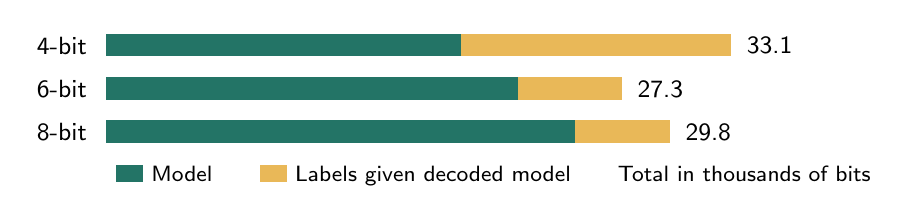
\begin{tikzpicture}[x=.24cm,y=.55cm,font=\sffamily\small]
\foreach \y/\b/\w/\d/\total in {2/4/18.800/14.290/33.1,1/6/21.792/5.517/27.3,0/8/24.800/5.047/29.8}{
\node[anchor=east] at (-.5,\y+.25){\b-bit};
\fill[sea] (0,\y) rectangle (\w,\y+.52);
\fill[gold] (\w,\y) rectangle (\w+\d,\y+.52);
\node[anchor=west] at (\w+\d+.3,\y+.25){\total};}
\node[anchor=west,font=\sffamily\footnotesize] at (0,-.75){\textcolor{sea}{\rule{10pt}{6pt}} Model\qquad \textcolor{gold}{\rule{10pt}{6pt}} Labels given decoded model\qquad Total in thousands of bits};
\end{tikzpicture}
\end{center}
Six bits gave the shortest message. Moving from four to six made the network more expensive to send, but its predictions improved enough to save nearly 8,800 bits on the labels. Moving from six to eight saved only another 470 bits on labels and added 3,008 bits to the model. The architecture and parameter count stayed the same throughout.
\head{What we want to find out}
When a measure says one network is more complex than another, does it also tell us which one will generalize worse? The six-bit result answers a narrower question about the cost of describing labels we already have. To answer the bigger one, we would keep some labels aside, rank the networks by each measure and see how that ranking lines up with their error on the held-out labels. Parameter count gives us a baseline.
\head{Why it matters}
Imagine two checkpoints of the same network that make equally good predictions on the training set. One still predicts well after we round its weights. The other starts making confident mistakes. Counting weights gives them a tie. Encoding them shows where their behaviour differs and suggests something concrete to check on new examples.
\head{Follow along}
You can try the library on four observations. From a copy of the \href{https://github.com/intsystems/dl-complexity}{DL Complexity repository}, run
\begin{verbatim}
python -m pip install -e .
python examples/quickstart.py
\end{verbatim}
Look for the units beside each number. BIC gives you a score on the criterion's own scale. The two-part code gives you the length of a message.
\end{document}
